%
% VBrowser
%

\chapter{Using the VBrowser}
\label{chap:vbrowser}

\section{Starting the VBrowser} 

\subsection{VBrowser panel overview} 

 \begin{figure}[htbp]
 \centerline{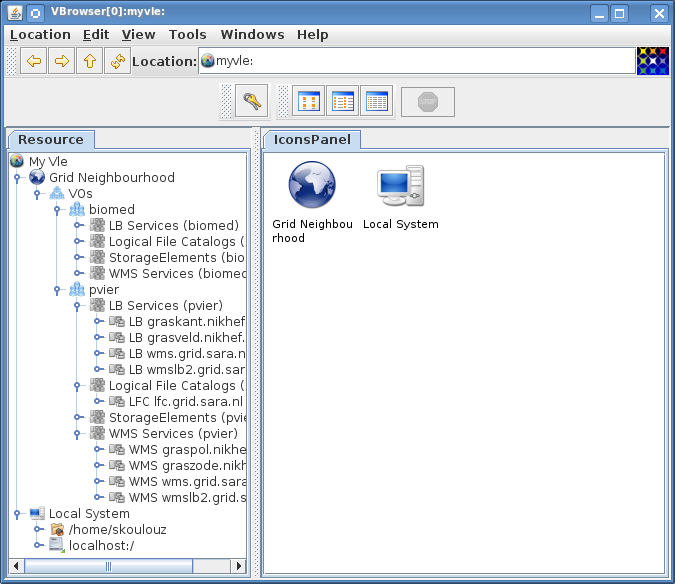
\includegraphics[scale=0.5]{vbrowser_main}}
 \caption{VBrowser window}
 \label{fig:vbrowser_window}
 \end{figure}
 
 
\subsubsection{Resource Tree panel} 
\label{section:resourcetree_panel}
 In the ResourceTree (Figure \ref{fig:vbrowser_window} left panel) in the upper 
 left there is the main resource or root resource called \myvle\ (You can rename 
 this resource). Directly below \myvle\ you can see the \GridHood\ containing 
 your VOs and the resources associated with them (see Section \ref{GridHood}). 
 Under that there is the \LocalSys\ with your home directory. All the resources in 
 this tree represent a logical ordering of your resources. When clicking on a tree 
 node the VBrowser will connect to the remote server or resource and 'open' the 
 location. If the user doesn't click on the node or expands the tree the remote 
 server or resource will not be opened and no connection is used. Some actions might 
 require that the user first has opened the resource. 
 \\

\subsubsection{Icons panel} 
\label{section:icons_panel}
 The icons panel is by default the panel you see on the right when starting the
 \vbrowser.


\subsubsection{Actions}  
 Double click (Action Click) on the resources (their icons) to open these
 location or right click (or use alternative mouse button) to view and/or edit the properties of
 these resources. 
\par
 You can add new resources by right-clicking (or use alt-mouse-button)  on
 \myvle\ and select \Menu{new}. This also works by right clicking
 (alt-mouse-button) on the white space between the icons or \emph{canvas} in
 the IconsPanel on the right. 
\\

\subsubsection{Menu Bar}
The menu bar has six menus: 
\begin{itemize}
  \item \Menu{Location}. This includes sub-menus like New Window, Open, Close, etc.
  \item \Menu{Edit}, with cut, copy, paste, etc.
  \item \Menu{View}. This includes sub-menus like \Menu{View as Icons} or \Menu{List}, and \Menu{Preferences}. With the \Menu{Preferences} sub-menu the user can change between single and double click mouse behaviour.
  \item \Menu{Tools} which contain the VLTerm, a terminal for SSH and bash sessions (see Section \ref{section:vlterm}) as well as some external tools.
  \item Finally there is \Menu{Windows} and \Menu{Help} used to close wind getting help and debug respectively.
\end{itemize}
 
\subsection{Location and navigation bar}
\label{section:location_bar}

 The location bar is the place or location which you are currently viewing. It
 has standard navigation buttons like \emph{Back}, \emph{Forward}, \emph{Up} and
 \emph{Refresh}. 
 
  \begin{figure}[htbp]
  \centerline{
\includegraphics[scale=0.5]{locationbar}}
  \caption{Location bar}
  \label{fig:locationbar}
  \end{figure}

You can drop icons and other URLs (or URI compatible strings) into this
location. For example you can drag windows icons (from your windows desktop) and
internet browser links (from for example Internet Explorer or Firefox) into this
location bar. 
Also you can start a drag from the mini icon in the location bar and drop
resources into the ResourceTree, IconsPanel or on your native desktop. 
The action of a VBrowser to native desktop Drag and Drop (DnD) might depend
how your local operating settings are configured. \\
You can also drag files directly from your local desktop into the ResourceTree
and IconsPanel windows. 
\\
\subsubsection{Navigation Buttons}

Here is an overview of the navigation buttons:

 \begin{itemize}
  \item  
\includegraphics[scale=0.5]{refresh_icon} 
	Refreshes the current viewed location. 
  \item  
\includegraphics[scale=0.5]{browse_back_icon}
    Browses back one location from history.
  \item  
\includegraphics[scale=0.5]{browse_forward_icon}
    Browses a location forward again, when the user has browsed back.
  \item  
\includegraphics[scale=0.5]{browse_up_icon}
   Browse to the parent location of the current viewed location. 
   
 \end{itemize}
 
\subsection{Toolbars}
\label{section:toolbars}

 Toolbars are the bars which have a set of buttons with small icons in them. 
 These buttons represent menu shortcuts or optional ways to view the contents
 of a location. 

  \begin{figure}[htbp]
  \centerline{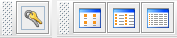
\includegraphics[scale=0.5]{toolbar}}
  \caption{Toolbars in the VBrowser}
  \label{fig:toolbars}
  \end{figure}

 An overview of the current toolbar buttons is as follows: 
 
 \begin{itemize}
 \item  
\includegraphics[scale=0.5]{invalid_creds_icon}
   Grid Credentials button. Status is invalid: Grid proxy has not been
   created.
 \item  
\includegraphics[scale=0.5]{valid_creds_icon}
    Grid Credentials button. Status is valid: Grid proxy has been created.
 \item  
\includegraphics[scale=0.5]{icons_icon}
   Icons panel button.
 \item  
\includegraphics[scale=0.5]{list_icon}
   List panel button. 
 \item  
\includegraphics[scale=0.5]{table_icon}
   Table panel button. 
\end{itemize}
  
Pressing the icon button will show the resources as icons, pressing the table
icons will present the resources in table with detailed information about the
resources. 

\subsection{Table panel}
\label{section:table_panel} 

When clicking on the table panel icon details from the resources will be
shown in a table form as can be seen in Figure  \ref{fig:table_panel}. 

\begin{figure}[htbp]
\centerline{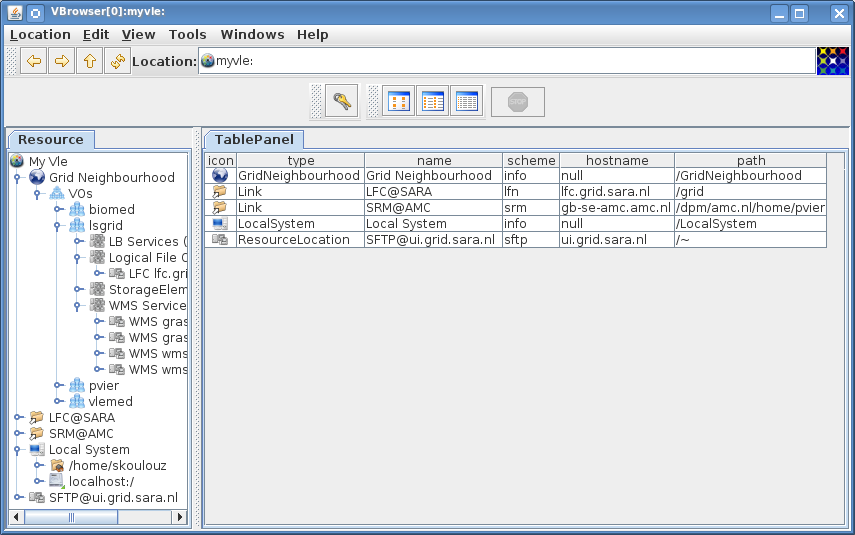
\includegraphics[scale=0.5]{table_panel}}
\caption{Table Panel}
\label{fig:table_panel}
\end{figure}

For each resource the default attributes are shown. 
Clicking on the header of the table column will sort the table according to the
logical value of the fields in that column. \\
More attributes can be added by right-clicking (or pressing alt-mouse button) on
the headerbar of the table panel as can be seen in 
Figure \ref{fig:table_panel_add_attributes}.\\


\begin{figure}[htbp]
\centerline{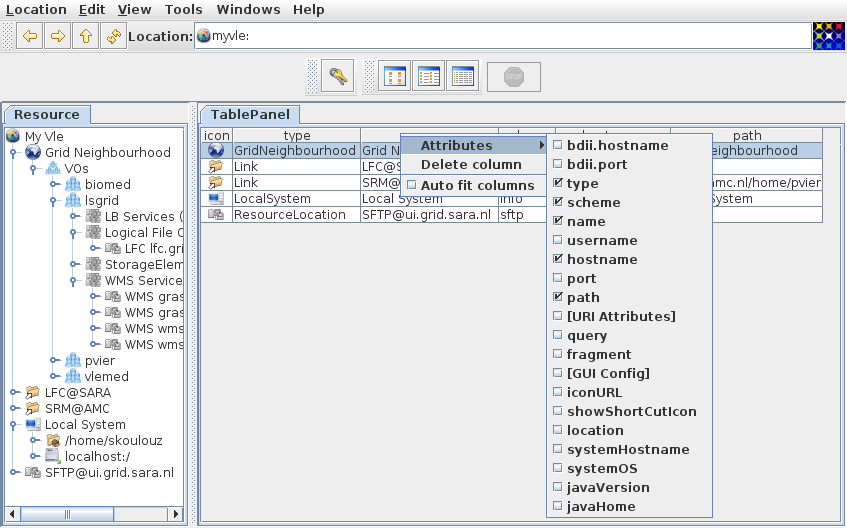
\includegraphics[scale=0.5]{table_panel_add_attributes}}
\caption{Table Panel with Attributes menu}
\label{fig:table_panel_add_attributes}
\end{figure}

You can also move around the columns by dragging the column header to the 
desired position. 
Currently the layout of the table is not saved between browsing sessions. 

\subsection{Pop-up or Action menu}

When right-clicking (or use alternative mouse button) on a resource, an pop-up
menu will appear. This is the Resource's Action Menu and from this menu special
actions can be selected which are to be performed on the resource. 
These actions include standard \Menu{Copy} and \Menu{Paste} actions as well as 
more complicated actions. See Figure \ref{fig:vbrowser_action_menu}

 \begin{figure}[htbp]
  \centerline{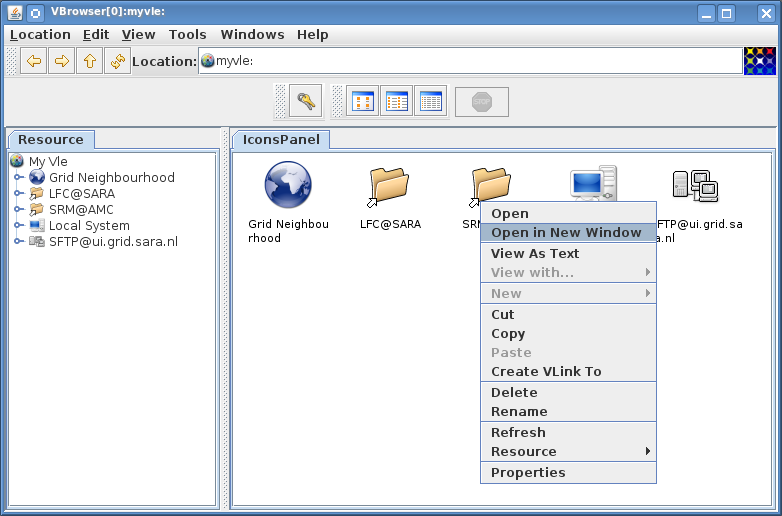
\includegraphics[scale=0.5]{vbrowser_action_menu}}
  \caption{VBrowser Action Menu}
  \label{fig:vbrowser_action_menu}
 \end{figure}
  
 \section{Authenticating yourself with the Grid} 
 \label{section:auth}

The first thing you do is to authenticate yourself with the grid. This is done
by creating a \Emph{grid proxy certificate} which is a file containing a temporary key which
you must use to access resources on the grid. 
For security reasons this file can only be used for a limited time. \\
To create a grid proxy you can use your \Emph{Grid Certificate} and your secret
\Emph{Passphrase} which combined can create a Grid Proxy for you. \\
To create one interactively,  click on the \Emph{keys} icon which can be seen in
Figure \ref{fig:grid_proxy_icon}. 

 \begin{figure}[htbp]
  \centerline{
\includegraphics[scale=0.5]{invalid_creds_icon}}
  \caption{Grid Proxy Icon}
  \label{fig:grid_proxy_icon}
 \end{figure}

A dialogue will appear where you can create your grid proxy. See Figure: 
\ref{fig:grid_proxy_init_dialog}. 

 \begin{figure}[htbp]
  \centerline{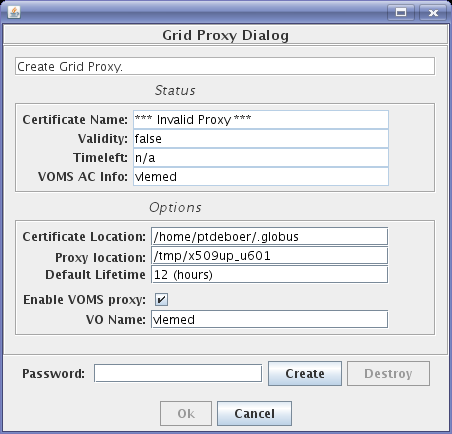
\includegraphics[scale=0.5]{grid_proxy_init}}
  \caption{Grid Proxy Creation Dialogue}
  \label{fig:grid_proxy_init_dialog}
 \end{figure}

To create a Grid Proxy, enter your passphrase and press \Menu{Create}. Your
grid proxy will be valid for 12 hours if not specified otherwise. Also to be 
able to use resources assigned to your VO, you would have to enable the 
\Menu{VOMS proxy}\footnote{VO: Virtual Organization. VOMS: Virtual Organization 
Management Service} option and fill in your VO name. More information about 
VOs may be found here: \cite{foster:2001:grid-anatomy,springerlink:10.1007/978-3-540-24689-3_5}
You can enter grid proxy creation options, like proxy location (file path) and
lifetime (in hours), in the dialog if needed. Also you can \Menu{Destroy} 
your grid proxy if you don't need it any more. Pressing \Menu{Create} again will 
refresh your proxy and update it with a new lifetime.\\

\section{Grid Neighbourhood}
\label{section:grid_hood}
 The \GridHood\ is a collection of Grid Resources (File Catalogue,Storage Elements,etc.) 
 grouped by VO. It can be configured using the property panel specifying the host and port of the BDII 
 service to query \cite{cite:bdii,cite:gridinfo}. 

 \begin{figure}[htbp]
  \centerline{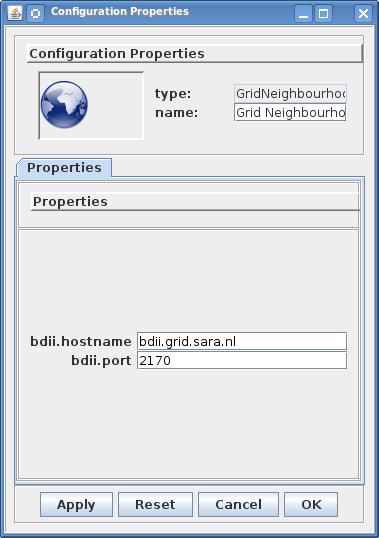
\includegraphics[scale=0.5]{gridHood_properties}}
  \caption{\GridHood\ properties}
  \label{fig:gridHood_properties}
 \end{figure}

 This resource seen in Figure \ref{fig:grid_hood} is organized as following: 
\begin{itemize}
  \item \GridHood\ . The top level resource.
  \item \VOGroup\ . The collection of VOs the user is part of. Each time the user authenticates 
                    him self having the \Menu{VOMS proxy} enabled, a new \VOGroup\ is created. 
                    Alternatively the user can create a new \VOGroup\ manually, by pressing \rightclick\ ,
                     \Menu{New}, \Menu{VO}. Moreover the current active VO is indicated with a different 
                     icon (see Figure \ref{fig:selected_vo_icon}).
  \item \VO\ . The collection of resources that this VO has at its disposal.
\end{itemize} 

 \begin{figure}[htbp]
  \centerline{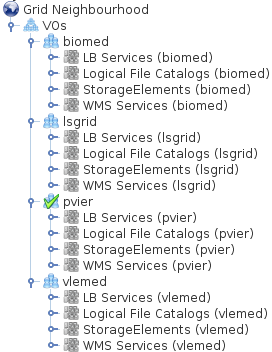
\includegraphics[scale=0.5]{grid_hood}}
  \caption{\GridHood\ Resource hierarchy}
  \label{fig:grid_hood}
 \end{figure}

%%
%% Note: selected_vo_icon is larger (128 pixels) then other (48 pixel)
%% 
 \begin{figure}[htbp]
  \centerline{
\includegraphics[scale=0.25]{selected_vo_icon}}
  \caption{The icon for the selected VO}
  \label{fig:selected_vo_icon}
 \end{figure}
 
Section \ref{section:configuring_myvle} describes how to add more resources, that might not be published by the BDII service as well as how to customise resource settings.

\section{Configuring your personal environment}
\label{section:configuring_myvle}

 When the \vbrowser\ starts, the left panel will show the Resource Tree with
 as first entry the 'Root Resource' currently named:  \myvle. 
 This root resource will contain your personal grid environment. You can rename
 this 'Toplevel Resource' to your any name you want. 

\subsection{Adding Resources} 
\label{section:adding_resources} 

 To add resource to your root resource, do the following:

	\step \rightclick\ on \myvle\ and select:\Menu{New}
	
	\step Select the resource you want to add. 


 \begin{figure}[htbp]
 \centerline{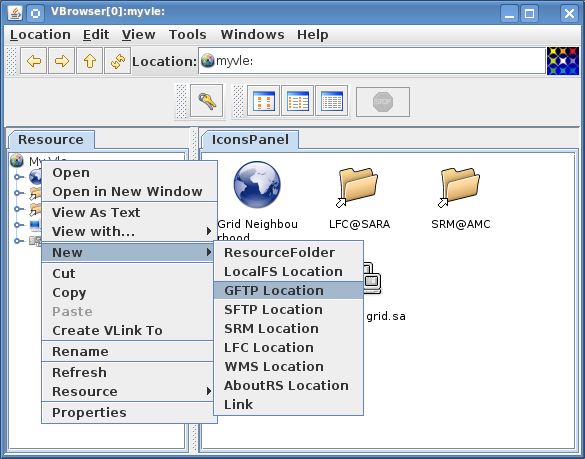
\includegraphics[scale=1]{myvle_new_server}}
 \caption{Create new location}
 \label{fig:myvle_new_server}
 \end{figure}

Deleting can be done as follows:\\
\\
\step \rightclick\ on the resource icon you want to delete and 
select:\Menu{Delete}\\ 
\\
\Note{Note}: Deleting a resource from the root resource (\myvle) will delete
the entry, never the directory it points to.\\
\\
To configure the settings for a resource, select the properties from the
pop-up menu as follows:\\
\\
\step \rightclick\ on the resource icon and select:\Menu{properties}\\
\\
Check and optionally change the properties of this resource.
	
\subsection{Adding New (Grid) Resource Location} 
\label{section:adding_gftp_server}
 
You can add a new Grid Resource Location, for example a 'GridFTP' location as
follows:\\
\\
\step \rightclick\ on \myvle\ and select:\Menu{New} \rarr \Menu{GFTP Location}\\
\\
Now set the GridFTP Location by selecting the properties
option from the pop-up menu as follows: \\
\\
\step \rightclick\ on the GridFTP icon and select:\Menu{properties}\\
\\
\begin{figure}[htbp]
\centerline{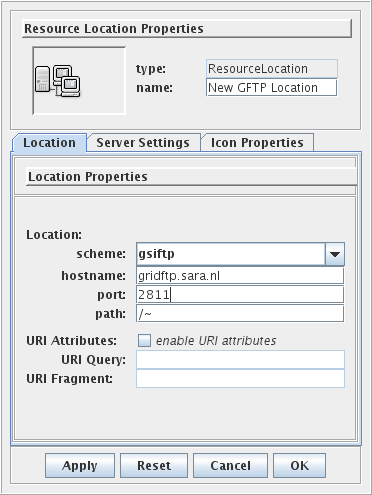
\includegraphics[scale=1]{gftp_location}}
\caption{GridFTP Location}
\label{fig:gftp_location}
\end{figure}
\\
Fill in the location of the new GridFTP server.
\\
\begin{itemize}
\item \Emph{scheme} : the scheme to use. For GridFTP leave this to 'gsiftp'.
\item \Emph{host}  : the hostname of the GridFTP location. 
\item \Emph{port}  : the port of the GridFTP location. The default value is
'2811'
\item \Emph{path}  : The path to start browsing. Leave to '$\sim$' to use
your default home location on the remote server. 
\item \Emph{URI properties}  : Not supported for GridFTP. 
\end{itemize}

To configure the server properties for this location, click on the \Menu{Server
Settings} tab and specify the settings for this server. 
\\
\begin{figure}[htbp]
\centerline{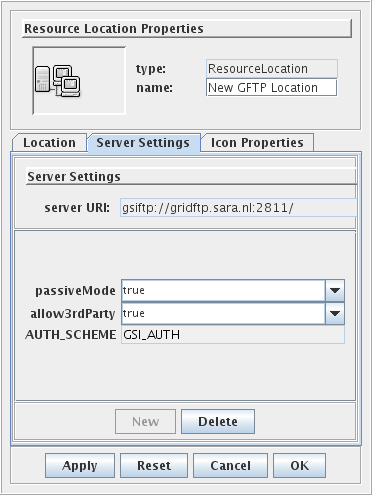
\includegraphics[scale=1]{gftp_properties}}
\caption{GridFTP Server Settings}
\label{fig:gftp_properties}
\end{figure}
\\
Current Server Settings for GridFTP servers are:
\begin{itemize}
\item \Emph{passiveMode} : set to 'true' when incoming connections are not
possible, for example when browsing from behind a firewall. 
\item \Emph{allow3rdParty} : whether 3rd party copying is possible to and from
this server.  This is used when copying between two (remote) Grid FTP locations.  
\end{itemize}

\subsection{Adding an LFC Location} 
\label{section:adding_lfc_server} 

To create an LFC \cite{10.1109/HPDC.2005.1520941} location do as follows:

	\step \rightclick\ on \myvle\ and select:\Menu{New} \rarr \Menu{LFC
	Location}

 After creating a new location the resource properties editor should pop-up. 
 You can also manually edit these properties by selecting the edit properties
 option from the pop-up menu as follows: 

	\step \rightclick\ on the LFC icon and select:\Menu{properties} 

\begin{figure}[htbp]
\centerline{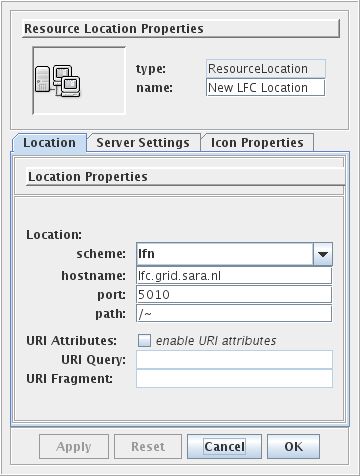
\includegraphics[scale=1]{lfc_location}}
\caption{LFC Location}
\label{fig:lfc_location}
\end{figure}

Fill in the location of the new LFC server.

\begin{itemize}
\item \Emph{scheme} : the scheme to use. For LFC leave this to 'lfn'.
\item \Emph{host}  : the hostname of the LFC server. 
\item \Emph{port}  : the port of the LFC server. The default value is '5010'
\item \Emph{path}  : the path to start browsing. Fore example '/grid/lsgrid' or 
                     use tilde: '$/\sim$' to auto resolve to you VO home location. 
                        
\item \Emph{URI properties}  : Not supported for LFC locations.  
\end{itemize}

 \begin{figure}[htbp]
  \centerline{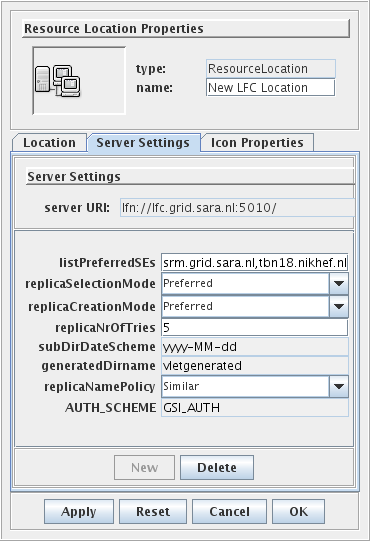
\includegraphics[scale=1]{lfc_properties}}
  \caption{LFC Server Settings}
  \label{fig:lfc_properties}
 \end{figure}

To specify the server configuration for this location, click on the
\Menu{Server Settings} tab and specify the settings for this server. 
Here an overview of the LFC settings:

\begin{itemize}
\item \Emph{listPreferredSEs} : list of Preferred Storage Elements to
use when selecting a replica to read from or when creating a new replica. This
is a comma seperated list of hostnames which can have an optional port number. 
\item \Emph{replicaSelectionMode} : replica selection algorithm used when
there is more then one replica to choose from (used when reading an
LFC file).
\item \Emph{replicaCreationMode} : Storage element selection algorithm
used when creating new replicas (used when uploading or writing to an LFC file). 
\item \Emph{replicaNrOfTries} : number of attempts tried when selecting a
replica to read from or when creating a new replica at a Storage Element. A
minimum of 3 is recommend or the number of replicas+1 if that if bigger than 3.     
\item \Emph{generatedDirname} : parent directory which will be used
at a Storage Element for all generated replicas. This directory name will be
appended to the default VO writeable location or VO Storage Area (see
explanation below).
\item \Emph{subDirDateScheme} : sub directory syntax used when
replicas are created in the replica parent directory: \Emph{generatedDirname}
(see explanation below).
\item \Emph{replicaNamePolicy} : file name policy when creating replicas at
Storage Elements (see explanation below). 
\end{itemize}

Each of the above server properties is explained more in details below: 

\subsubsection{List of Preferred Storage Elements (listPreferredSEs) } 

The server property \Emph{listPreferredSEs} is a comma seperated list of
hostnames which contains the user preferred Storage Elements. 
This list is used when uploading a file to an LFC server to choose a
Storage Element to store a replica.  
When downloading a file, this list is used to select a replica witch matches a
Storage Element from this list. How this matching occurs depends on 
the \Emph{replicaSelectionMode} or the \Emph{replicaCreationMode} settings.    

\subsubsection{Replica Selection Algorithm (replicaSelectionMode) } 

The option \Emph{replicaSelectionMode} determines which algorithm is used when
selecting a replica to read from. This is one of the following: 

\begin{itemize}
  \item \Emph{Preferred}$^1$ :  Try to find a replica which matches one of the
  hostnames listed in the server property which specified the list of preferred
  Storage Elements: \Emph{listPreferredSEs}. 
  The order in which replicas are tried is the same as the order of the
  hostnames in this list. 
  \item \Emph{PreferredRandom}\footnote{} : Same as \Emph{Preffered} but the list of
  matching replicas is randomized. 
  \item \Emph{AllSequential} : Try all replicas in order as they are registered
  at the LFC server. The first that is available will be used. If all replicas
  have been tried, the selection procedure will start with the first until the
  maximum number of tries has been reached. 
  \item \Emph{AllRandom} : Same as \Emph{AllSequential} but the order in which
  replicas are tried is randomized. As this randomization is 'true' random,
  same replicas might be tried twice in a row. This is by design. 
\end{itemize} 

\Note{$^1$} If no replicas match the list of preferred Storage Elements
(\Emph{listPreferredSEs}) or this list is empty, the mode \Emph{AllSequential}
will be used.

\subsubsection{Replica Creation Algorithm (replicaCreationMode) }

The option \Emph{replicaCreationMode} determines which algorithm is used when
selecting a Storage Element to create a replica. 
This is one of the following:

\begin{itemize}
  \item \Emph{Preferred} :  Only the Storage Elements from the 
      \Emph{listPreferresSEs} list are use to create a new Replica. The order in
      which Storage Elements are tried is the same as the order of the list. 
  \item \Emph{PreferredRandom} : Same as \Emph{Preferred} but the list will be
      randomized. Since the randomiser is 'true' random, a Storage Element
      might be tried multiple times even if it has already been tried before
      unless it already has a replica. 
  \item \Emph{DefaultVORandom} : A Random Storage Element is used from the list
  of allowed Storage Elements for the current user's VO by querying the grid info
  service (BDII). If this Storage Element fails another is randomly selected.   
\end{itemize} 
 
\subsubsection{Replica number of Tries (replicaNrOfTries) } 

The number of attempts undertaken to either read a replica or the number of
attempts to create a replica at a Storage Element. 

\par
When reading from an LFC file (downloading), this number determines how many
times an attempt is made to read from any of the available replicas.
If, for example, the number of replicas is only 1, the same replica will be
tried each time. 
If the number of available replicas is less than the \Emph{replicaNrOfTries} the
same replica might be tried more then. Which replica is used depends on the
\Emph{replicaSelectionMode}.

\par
When uploading a file to LFC, this number determines how many times an
attempt is made to create a replica at one of the available Storage
Elements. Which Storage Element is used depends on the
\Emph{replicaCreationMode}.

\subsubsection{Replica directory and file name creation policy
(generatedDirname, subDirDateScheme, replicaNamePolicy) }

The options \Emph{generatedDirname}, \Emph{subDirDateScheme} and 
\Emph{replicaNamePolicy} determine which path is used when creating a replica
at a Storage Element.\\
The path is created by using the following syntax:\\
\\
\Path{ srm://\lt VO Storage Area\gt /\lt generatedDirname\gt/\lt
subDirDateScheme\gt/\lt replicaFileName\gt}\\
\\ 
The \Path{ \lt VO Storage Area\gt} is the VO allowed Storage Area which is
dynamically determined by querying the appropriate grid info service (BDII). 

The \Path{\lt replicaFileName\gt} is a generated file name which can resemble
the logical file name of the LFC entry the file is an replica for. This depends
on the \Emph{replicaNamePolicy} setting. \\
This can be one of the following:

\begin{itemize}
  \item \Emph{Random} : The filename is a randomized file name only.  
  \item \Emph{Similar} : The filename contains the original logical filename
  and a randomized identifier. 
\end{itemize}

Example of a \Emph{Random} replica file path at a storage element:\\
\\
\tab
\Path{
/pvier/vletgenerated/2009-07-01/file\_fad71348-d80b-48e5-bf2d-24590bb7c5f2
}
\\
\\
Example of a \Emph{Similar} replica file path for the LFC file with name
'experiment.txt' :\\
\\ 
\tab
\Path{ /pvier/vletgenerated/2009-07-01/experiment\_txt\_fad71348-d80b-48e5-bf2d-24590bb7c5f2
}
\\

% \subsection{Adding an SRB Location} 
% \label{section:adding_srb_server} 
%  To create an SRB location perform the following steps: 
%  
% 	\step \rightclick\ on \myvle\ and select:\Menu{New} \rarr \Menu{SRB
% 	Location}
% 
%  Now set the SRB location properties by selecting the properties option
%  from the pop-up menu as follows: 
%  
% 	\step \rightclick\ on the SRB icon (MySRB) and select:\Menu{properties}  
% 
%  \begin{figure}[htbp]
%   \centerline{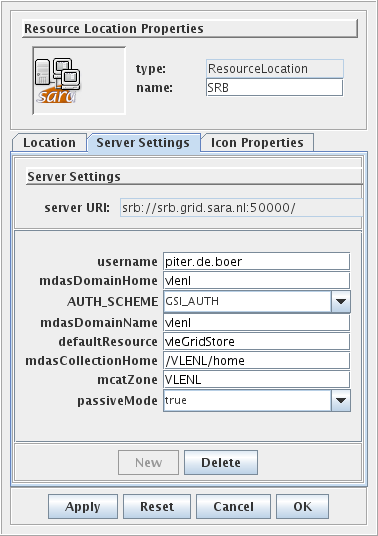
\includegraphics[scale=0.5]{srb_properties}}
%   \caption{SRB server properties}
%   \label{fig:srb_properties}
%  \end{figure}
% 
% Current Server Settings (Select the \Menu{Server Settings}  tab) for SRB servers
% are:
% \begin{itemize}
% \item \Emph{passiveMode} : set to 'true' when incoming connections are not
% possible, for example when browsing from behind a firewall. 
% \item \Emph{AUTH\_SCHEME} : authentication scheme. GSI authentication is the
% standard used on the Grid. 
% \item \Emph{mdas/mcat settings} : Make sure you fill in the right
% \Emph{mdas}\ldots settings and \Emph{mcat}\ldots settings. Contact your SRB
% administrator for the right values. 
% \item \Emph{defaultResource} : A SRB Server might allow different values
% for the \Emph{defaultResource}. Contact your SRB administrator for the right
% values. (Values given are example values).
% \end{itemize}


\section{Links or shortcuts}
\label{section:links} 

 Another way of creating a resource entry is creating a \link. A \link\ behaves in
 a similar way as shorcuts on windows. This type of resource does \Emph{not} 
 resemble a Unix hard- of softlink in anyway. When opening a \link, the location 
 pointed to by the \link, will be opened. 
 
 Typically a \link\ icon has a small arrow in the bottom left corner
 to indicate it is a link, as can be seen in Figure \ref{fig:linkicon}.

 \begin{figure}[htbp]
  \centerline{
\includegraphics[scale=0.5]{linkicon}}
  \caption{Link icon}
  \label{fig:linkicon}
 \end{figure}

 You can create a link by selection the \Menu{Create VLink to} option from 
 the pop-up menu or action menu.